\documentclass[a4paper,10pt]{article}
\usepackage[utf8]{inputenc}
\usepackage[english]{babel}
\usepackage{graphics}
\usepackage{graphicx} %per le figure
\usepackage{subfigure} %per le figure
\usepackage{multirow}
\usepackage{geometry}
\usepackage{pdfpages}
\usepackage{esvect}
\usepackage{tikz,amsmath}

\author{Andrea Celentano\thanks{andrea.celentano@ge.infn.it}\\ \small{INFN, Sezione di Genova}}
\title{The reaction $\gamma^* p \rightarrow X \rightarrow J/\psi \, p$: a feasibility study in the MesonEx experiment at CLAS12}
\begin{document}
\maketitle
\begin{abstract}
We present a preliminary feasibility study of the measurement of the  $\gamma~p~\rightarrow~J/\psi~\,~p$ reaction in the MesonEx experiment at CLAS12. The main focus is the investigation of possible ``exotic'' $s-$channel resonances, decaying to the $J\psi \, p$ final state, such as the $P_c(4380)$ and the $P_c(4450)$ states recently claimed by the LHCB experiment. In this note we present the specific kinematics for this reaction, the expected detector performances in terms of acceptance and resolution, and an estimate of the foreseen number of measured events expected in the experiment.
\end{abstract}
\section{Introduction}

The LHCB experiment has recently reported \cite{Aaij:2015tga} the discovery of two $J/\psi \, p$ resonances in the decay $\Lambda^0_b\rightarrow J/\psi K^- p$ decay: the $P_c(4450)$ state, with mass $M_a=(4380 \pm 8 \pm 29)$ MeV and width $\Gamma_a=(205\pm18 \pm86)$ MeV, and the $P_c(380)$ state, with mass $M_b=(4449.8\pm1.7\pm2.5)$ MeV and width $\Gamma_b=(39\pm5\pm19)$ MeV. The reported statistical significance for these two states is, respectively, 12$\,\sigma$ and 9$\, \sigma$. The quantum numbers $J^P$ have been determined trough Partial Wave Analysis: the most probable solution was found to be $J^P_a=(3/2)^-$ and $J^P_b=(5/2)^+$, although the solution $J^P_a=(3/2)^+$ and $J^P_b=(5/2)^-$ was found to produce almost the same maximum likelihood value.

Immediately after the LHCB announcement, an intense debate started about the nature of these states. Many hypothesis have been proposed so far: a molecular-like state, formed by a charmed baryon and an anti-charmed meson  \cite{Chen:2015loa,Chen:2015moa,Roca:2015dva,He:2015cea}, a quark-diquark-diquark structure \cite{Maiani:2015vwa,Anisovich:2015cia}, a confined but rapidly separating color-antitriplet diquark and color-triplet triquark \cite{Lebed:2015tna}, a composite object made of the charmonium state $\chi_{c1}$ and the proton \cite{Meissner:2015mza}. Finally, some authors suggested that at least one of the two states is not a resonance, but a kinematical singularity due to rescattering in the  $\Lambda^0_b\rightarrow J/\psi K^- p$ decay \cite{Guo:2015umn,Liu:2015fea,Mikhasenko:2015vca}.

It has also pointed out that the expected cross-section for the direct photo-production of these states can be significantly large \cite{Karliner:2015voa,Wang:2015jsa,Kubarovsky:2015aaa}. In particular, focusing on the narrower state $P_C(4449)$, Karliner and Rosner \cite{Karliner:2015voa} estimated $\sigma \simeq 3.6~\mu$barn, while Wang, Liu and Zhao \cite{Wang:2015jsa} obtained  $\sigma \simeq 80$ nbarn. These calculations assume a branching fraction $B_o$ of the decay $X \rightarrow J/\psi~p$ equal to 1.

In this note, we consider the measurement of the reaction $\gamma^* p \rightarrow X \rightarrow J/\psi \, p$ in the MesonEx experiment at Jefferson Laboratory \cite{MesonEx}, discussing the foreseen kinematics, detector response, and number of expected events. For simplicity, we will focus on the study of the narrower state, the $P_c(4449)$.

\subsection{The MesonEx experiment}

\subsection{General features of the measurement of the $\gamma^* p \rightarrow X \rightarrow J/\psi \, p$ reaction in MesonEx}

Before discussing in details the measurement $\gamma^* p \rightarrow X \rightarrow J/\psi \, p$ reaction in the MesonEx experiment, we want to briefly discuss few general features, that show the high potentiality of this experiment searching for resonances decaying in the $J/\psi\, p$ final state. 

We consider the quasi-real photo-production reaction $e~p~\rightarrow~\gamma^*~p~e^{\prime}~\rightarrow~J/\psi~p~e^{\prime}$, with the final stat electron scattered at low angle and measured in the Forward Tagger detector. The final state proton and the $J/\psi$ decay products, instead, are measured in the CLAS12 detector.

In this analysis, we focused only in the $J/\psi$ decay to an electron-positron pair. We do not consider the $\mu^+ \mu^-$ decay channel, that as a comparable branching ratio, since the CLAS12 detector is not equipped with a muon identification system and, therefore, pion background would probably be too high to clearly identify the $J/\psi$ signal.


\paragraph{Invariant mass resolution: } the invariant mass $W$ of the $J/\psi\, p$ system can be measured in MesonEx as the missing mass of the final state electron, that depends only from the measured energy of the electron in Forward Tagger. Explicitly,
\begin{equation}
W^2=M_p^2+2E_0M_P-2E^{\prime}M_p \; \; ,
\end{equation}
with $E_0$, $E^{\prime}$ the primary beam energy and the final state electron energies. In particular, for $W=4449.8$ MeV (mass of the narrower $P_c$ state), $E^{\prime}=917.7$ MeV ($E^*_{\gamma}=10.08$ GeV). Therefore, close to the resonance mass,
\begin{equation}
\sigma_W=\sigma_{E^{\prime}} \cdot \frac{M_p}{W} \simeq 0.21 \cdot \sigma_{E^{\prime}} \simeq \mbox{ 5.2 MeV}\; \; ,
\end{equation}  
being $\sigma_{E^{\prime}} \simeq$ 25 MeV the expected energy resolution for the final state electron measured in the Forward Tagger Detector \cite{Celentano:2014boa}. This value is significantly lower than the resonance width reported by LHCB, $\Gamma_a=39$ MeV, demonstrating that the experiment will be capable of properly determining the resonance line-shape.
\paragraph{Number of measured events: } in the low $Q^{2}$ limit, the unpolarized differential reaction cross-section, with respect to the scattered electron angle $\Omega^{\prime}$ and energy $E^{\prime}$ in the laboratory frame, is \cite{Budnev:1974de}:
\begin{equation}
d\sigma(\Omega^{\prime},E^{\prime}) = \sigma_\gamma(\nu) \cdot d \Psi(\Omega^{\prime},E^{\prime}) \; \; ,
\end{equation}
with $\sigma_\gamma(\nu)$ the \textit{total} cross section for the real photo-production reaction $\gamma p \rightarrow J/\psi\, p$, being $\nu$ the virtual photon energy. The term $d \Psi(\Omega^{\prime},E^{\prime})$ is the equivalent photon flux, given by:
\begin{equation}
d\Psi(\Omega^{\prime},E^{\prime})=\frac{\alpha}{4\pi^{2}}\frac{E^{\prime}}{E_0}\frac{\nu}{Q^2}\left[\frac{(2E_0-\nu)^2}{\nu^2}+1  \right] d\Omega^{\prime} \,d E^{\prime}
\end{equation}
A slightly over-estimated estimate for the number of expected events can be obtained by assuming a constant photo-production cross-section $\sigma^{\gamma}_0$, equal to the value at the resonance mass, and integrating in the electron energy range corresponding to the mass interval $(M-\Gamma/2,M+\Gamma/2)$, i.e. 825.1 MeV $<$ $E^{\prime}$ $<$ 1010.0 MeV. The angular integration, instead, has to be performed over the Forward Tagger nominal acceptance, i.e. $2.5^{\circ}<\theta^{\prime}<4.5^{\circ}$, resulting in $\Psi=2.52\cdot 10^{-5}$.

The foreseen rate of produced events, considering the nominal MesonEx luminosity, $\mathcal{L}=10^{35} cm^{-2} s^{-1}$, is therefore:
 \begin{equation}
R_{gen} = \mathcal{L} \cdot \Psi \cdot \sigma^{\gamma}_0 \simeq 2 \cdot 10^5 \cdot \sigma^{\gamma}_0 \mbox{ events / day / }\mu{\mbox barn}
\end{equation}

To get the actual number of measured events, this has to be multiplied by the branching fraction for the decay $J/\psi\rightarrow e^{+} e^{-}$ ($\simeq 5.9\%$). Finally, the CLAS12 acceptance $\varepsilon$ has to be considered: as discussed below, the value obtained from MonteCarlo simulations is $\varepsilon \simeq 0.13$, if all the final state particles (proton and electron-positron pair) are detected, and slightly higher if only the two leptons are measured, the proton being reconstructed via missing mass technique. This gives:
\begin{eqnarray}
R_{meas} &=& R_{gen} \cdot BR_{J/\psi\rightarrow e^{+}e^{-}} \cdot \varepsilon \simeq 1.5 \cdot 10^{3}  \cdot \sigma^{\gamma}_0 \mbox{ events / day / }\mu{\mbox barn}\\
 N_{meas} &\simeq& 1.2\cdot10^5 \cdot \sigma^{\gamma}_0 / \mu\mbox{barn} \; \; \; ,
\end{eqnarray}
considering the nominal MesonEx run time of 80 days. 
\section{Kinematics}
 
To simulate the measurement of the reaction $\gamma^* p \rightarrow J/\psi \, p$ with the CLAS12+Forward Tagger detector, we generated a large set of events trough a model developed ``ad-hoc'', described in Appendix \ref{app:model}. Two contributions were considered:
\begin{itemize}
\item{A non-resonant production mechanism, parametrized via the $t-$channel exchange of a Pomeron trajectory. 
All the corresponding parameters, including the overall normalization, were tuned to reproduce the experimental data measured at higher energy  ($E_{\gamma} > 13$ GeV) \cite{Camerini:1975cy}. 
We note, however, that the extrapolation of the total cross-section from the higher energy range where experimental data exist to the MesonEx range, close to the threshold, is very sensitive to the choice of the parameters. 
Specifically, with the actual values we used, we got $\sigma_{NR}(E_{\gamma}=10 \mbox{ GeV} ) = 0.2 $ nbarn\footnote
{
We observe that this value is compatible with the range predicted in \cite{Brodsky:2000zc}, where a QCD-inspired calculation was performed.}.
} 
\item{A resonant production mechanism  , $\gamma^* p \rightarrow X \rightarrow J/\psi \, p$. In this note, we focused only on the narrower state reported by the LHCB experiment, $P_c(4450)$, leaving a proper study of the measurement feasibility as a function of the $X$ mass and width for the future. Furthermore, in the development of the production model, we only considered the $J^P$ assignment $(3/2)^-$, although we verified that this has a very limited impact on the foreseen experimental acceptance. 

This contribution is characterized by a single free parameter, the branching ratio BR of the decay $X \rightarrow J/\psi \, p$. The total cross section at the resonance peak reads: $\sigma_{R}(E_{\gamma}=10 \mbox{ GeV} ) = (BR)^{2}\cdot 1.3 \, \mu$barn. In this note, we considered the case BR $\simeq$ 0.1, so that $\sigma_{R}~\simeq~60~\cdot~\sigma_{NR}$ at the resonance mass.}
\end{itemize}

The distribution of the  $J/\psi \, p$ invariant mass ($W$) is reported in Fig.~\ref{fig:1}, together with the correlation between $W$ and the momentum transferred on the proton, $-t$. In the production model that we developed, as described in Appendix~\ref{app:model}, the $X\rightarrow J/\psi \, p$ decay is almost isotropic in the CM frame, due to the barrier-factor effects in the proximity of the $J/\psi \, p$ threshold. The non-resonant contribution, instead, is characterized by a diffractive-like $t$ dependence, $d\sigma / d t~\propto~\exp(- b \cdot |t|)$, with $b\simeq 2.8$ \cite{Camerini:1975cy}.

The momentum-against-angle distribution for proton and leptons, in the laboratory frame, is plotted in Fig.~\ref{fig:2}. The proton is always emitted at low angle, $\theta_P < 25^{\circ}$, due to the lower mass with respect to the $J/\psi$ meson. The $e^{+}$ and the $e^{-}$, instead, are typically emitted at larger angle, with a significant fraction of events with one or both out of the CLAS12-FD acceptance.
\begin{figure}[tpb]
\subfigure{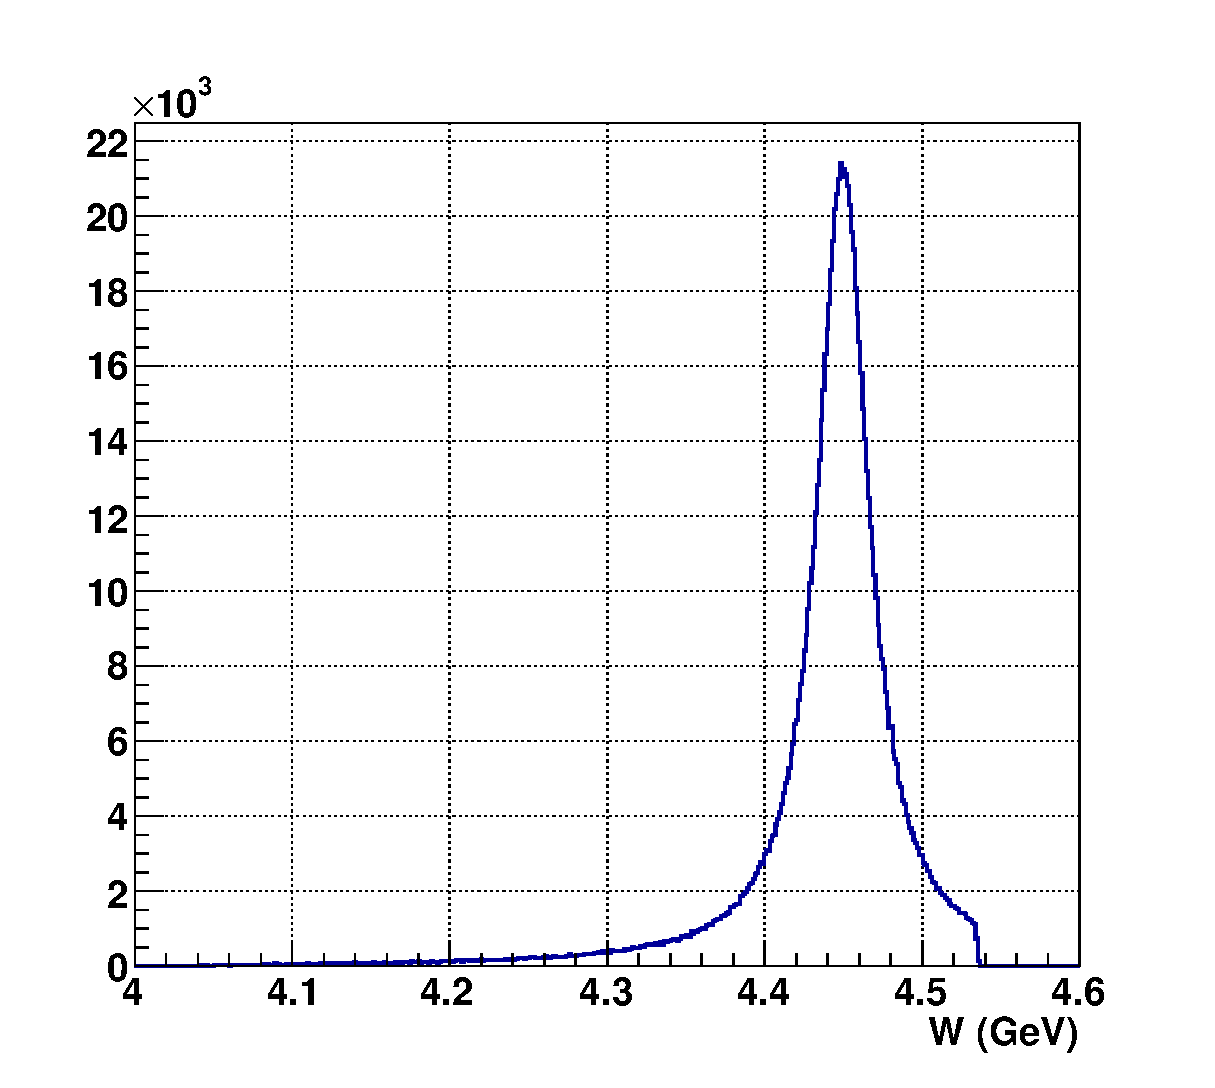
\includegraphics[width=0.45\textwidth]{WGEN.eps}}
\subfigure{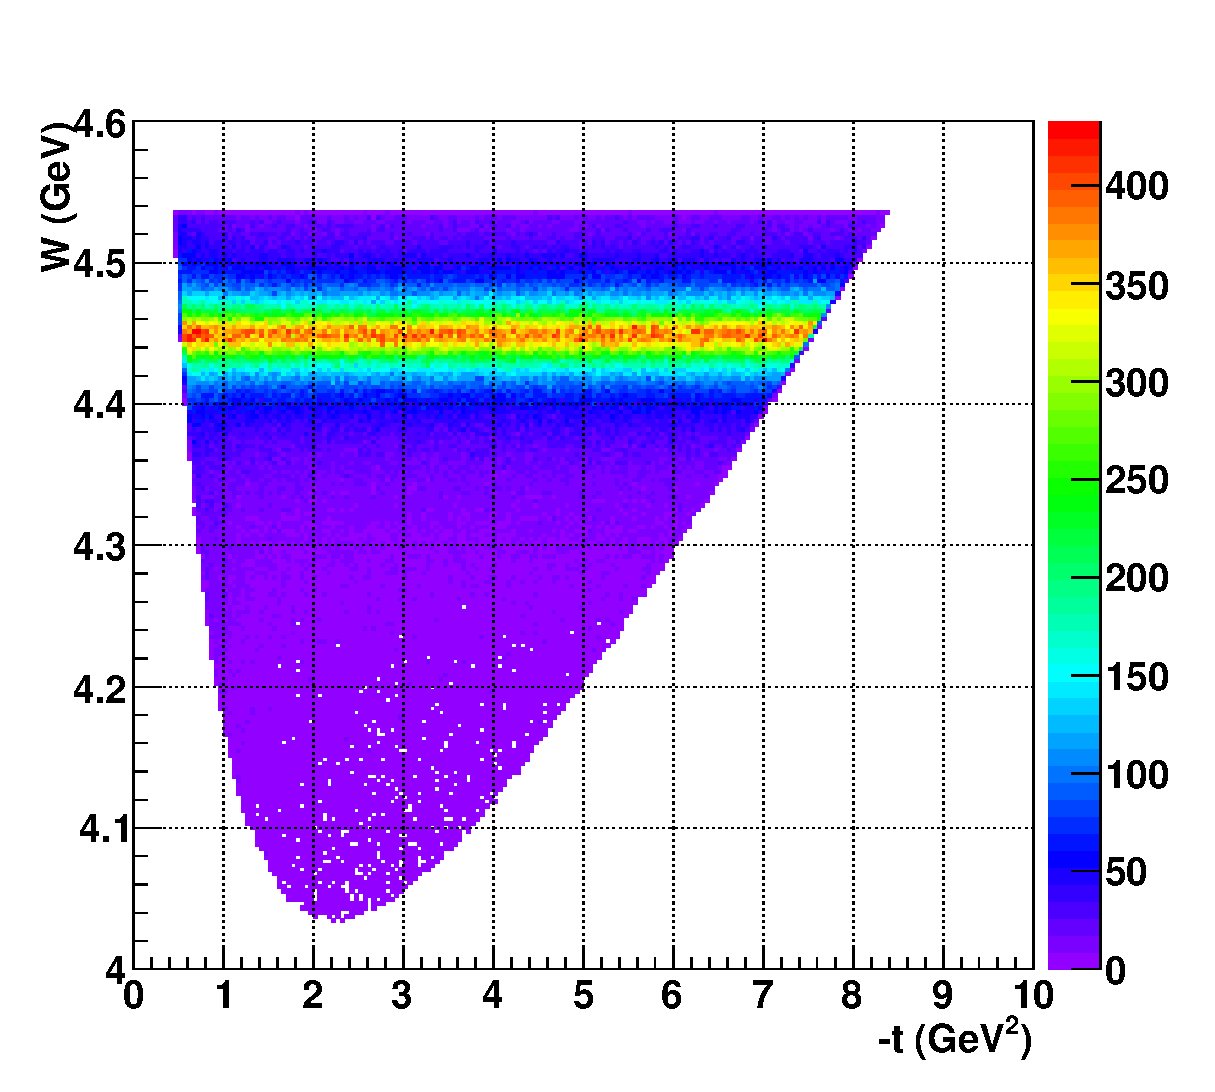
\includegraphics[width=0.45\textwidth]{WvstGEN.eps}}
\caption{\footnotesize \label{fig:1} Left: $J/\psi \, p$ invariant mass distribution. Right: $J/\psi \, p$ invariant mass vs momentum transfer on the proton distribution.}
\end{figure}

\begin{figure}[tpb]
\subfigure{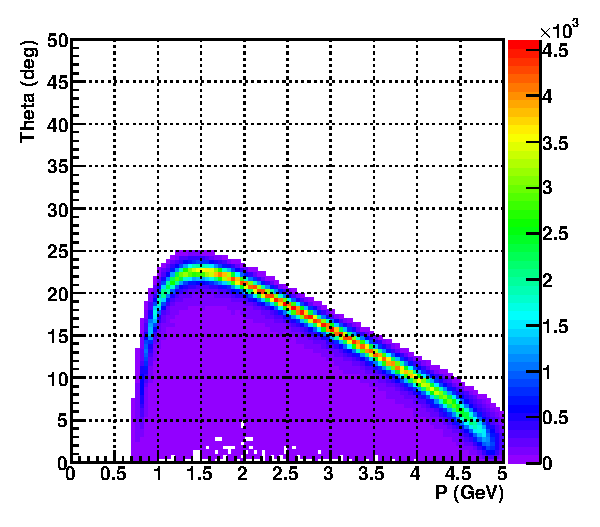
\includegraphics[width=0.45\textwidth]{protonGEN.eps}}
\subfigure{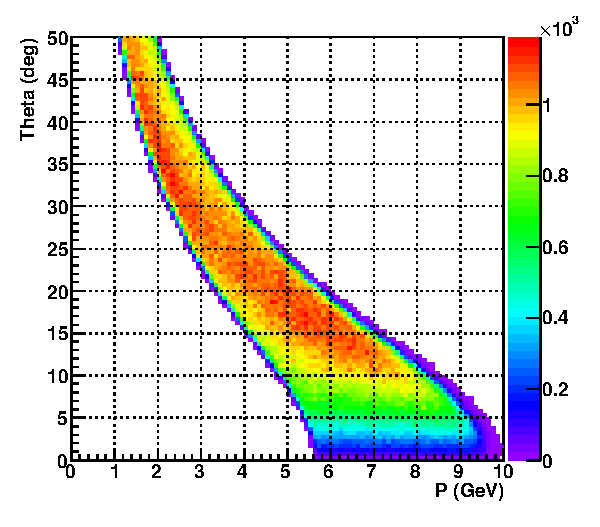
\includegraphics[width=0.45\textwidth]{leptonGEN.eps}}
\caption{\footnotesize \label{fig:2} Momentum-against-angle distribution for the final state proton (left) and for the leptons (right), in the laboratory frame.}
\end{figure}


\section{Detector response}

The reaction that we consider foresees 4 particles in the final state: a low-angle scattered electron, measured with the Forward Tagger facility, and a proton and an electron-positron pair from $J/\psi$ decay, measured with the CLAS12 detector. Since the CLAS12-Central Detector (CD) is not suited for electron detection and identification, we consider only the detection of final state leptons in the CLAS12-Forward Detector (FD). Two possible measurement strategies are possible:
\begin{itemize}
\item{Measure \textit{all} the final state particles, reconstructing the $J/\psi$ via the invariant mass of the electron-positron pair.}
\item{Measure \textit{only} the scattered electron in the Forward Tagger and the electron-positron pair in CLAS12-FD, reconstructing the $J/\psi$ via the invariant mass of the $e^{+} e^{-}$ system and the proton via the missing mass on it.}
\end{itemize} 
While the first solution would permit a better background discrimination, given the larger control on kinematics variable that the full measure of the final state permits, the second results in a slightly larger experimental acceptance. A proper discussion on the best measurement strategy would require a full simulation of the backgrounds associated with the measurement, not performed in this note: for this reason, in the following we will discuss both strategies. 

The CLAS12 and Forward Tagger response was simulated using the Fast MonteCarlo (FASTMC) software, that effectively accounts for the detector geometrical acceptance and resolution. Each final state particle, i.e. the recoil
proton, the scattered electron, and the two leptons, is projected individually on the detector. If it is within the nominal detector acceptance region, the four-momentum is smeared according to the expected resolution, otherwise it is discarded. We made the following conservative assumptions:
\begin{itemize}
\item{The CLAS12-CD acceptance for leptons is zero. As discussed, this reflects the fact that this detector is not designed for $e^- / e^+$ detection and identification.}
\item{We considered only events with both the electron and the positron from $J\/psi$ decay detected in the CLAS12-CD, i.e. we neglected the possibility that they are measured with the Forward Tagger.}
\end{itemize}

The resolution on the reconstructed $J/\psi$ mass, from the $e^{+} e^{-}$ measured four vectors, is reported in Fig.~\ref{fig:3}. At the maximum value of the CLAS12 toroidal field, with positive (negative) particles being outbended (inbeded), a resolution of $\simeq 15$ MeV is obtained, as shown in the left panel. The right panel, instead, reports the resolution on the $e^- - e^+$ missing mass, relevant for the second measurement strategy outlined before.

\begin{figure}[tpb]
\subfigure{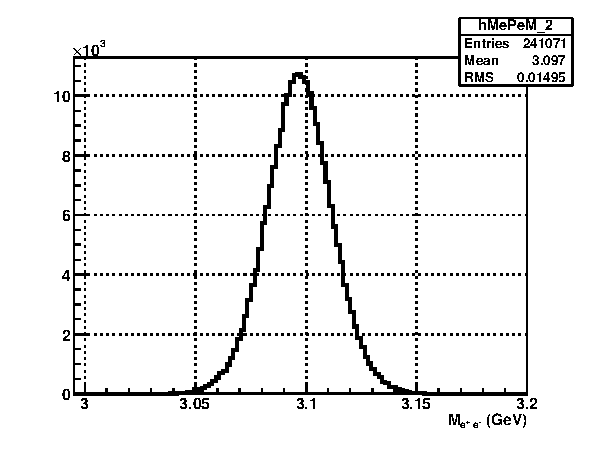
\includegraphics[width=0.45\textwidth]{resJPSInominal.eps}}
\subfigure{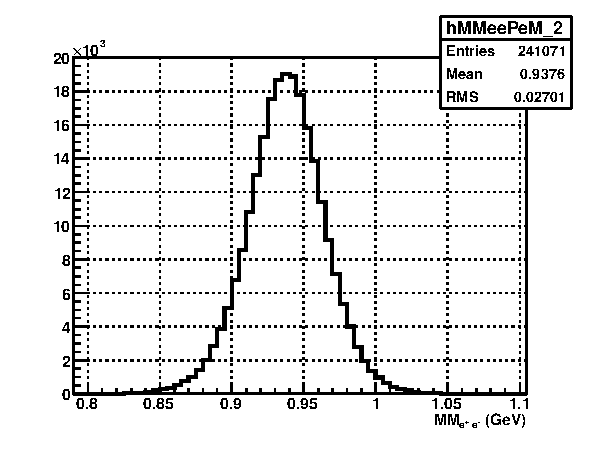
\includegraphics[width=0.45\textwidth]{resPnominal.eps}}
\caption{\footnotesize \label{fig:3} Left: reconstructed $J/\psi$ mass. Right: missing mass on the $e^+\,e^-$ pair. Both plots refer to the maximum value of the CLAS12 toroidal field, configured to have positive particles outbending.}
\end{figure}

We also investigated the effect of a magnetic field variation on the above quantities. As expected, we observed that there is almost no dependence on the orientation of the CLAS12 toroidal field, given the charge symmetry of the $e^+ e^-$ system. Results are reported in Fig.~\ref{fig:4}.

\begin{figure}[tpb]
\subfigure{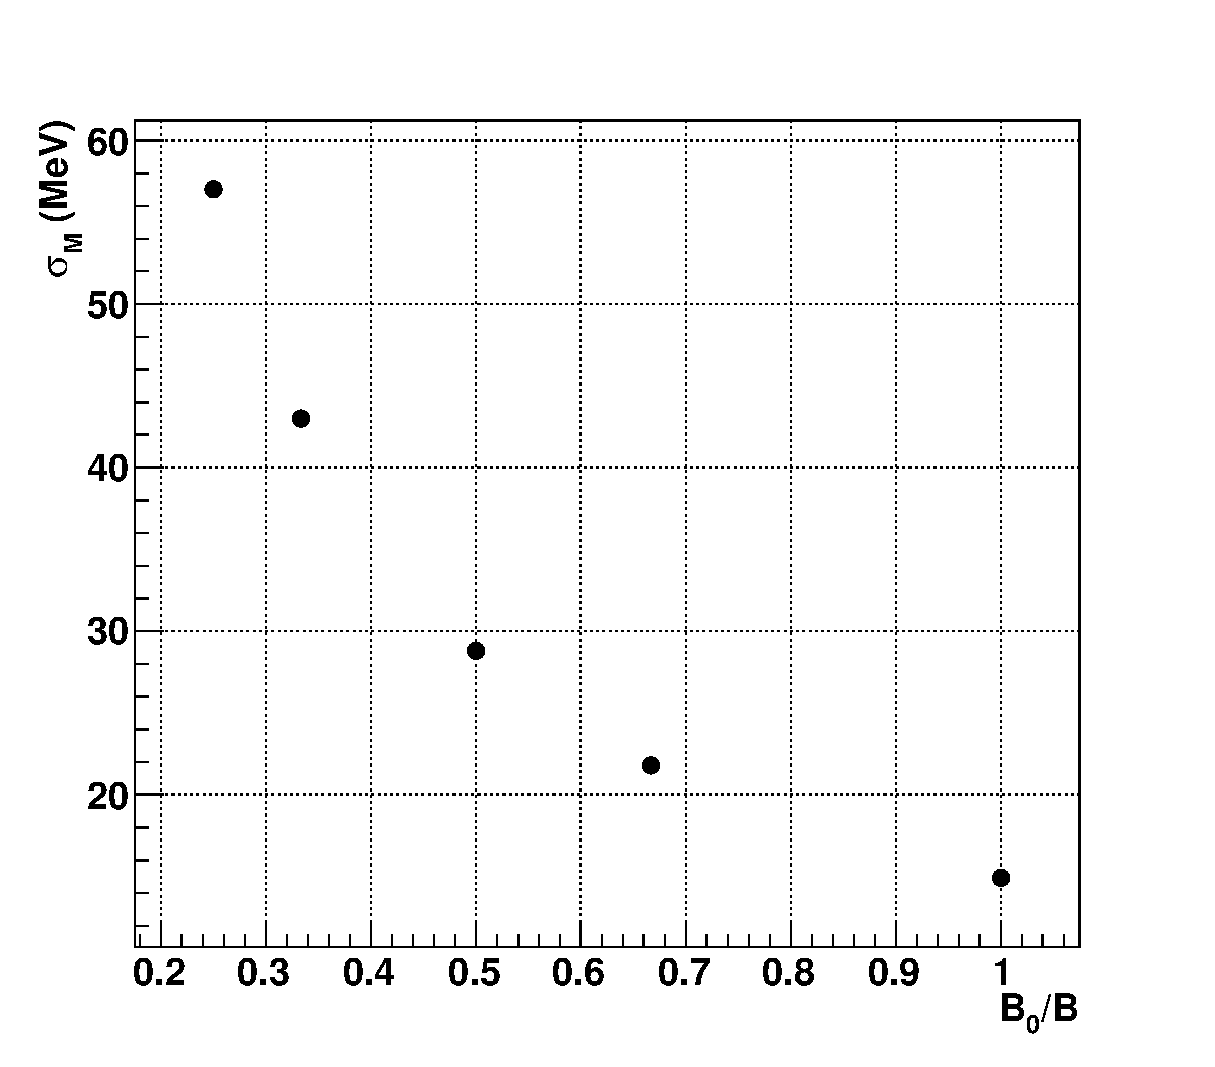
\includegraphics[width=0.45\textwidth]{resJPSIfield.eps}}
\subfigure{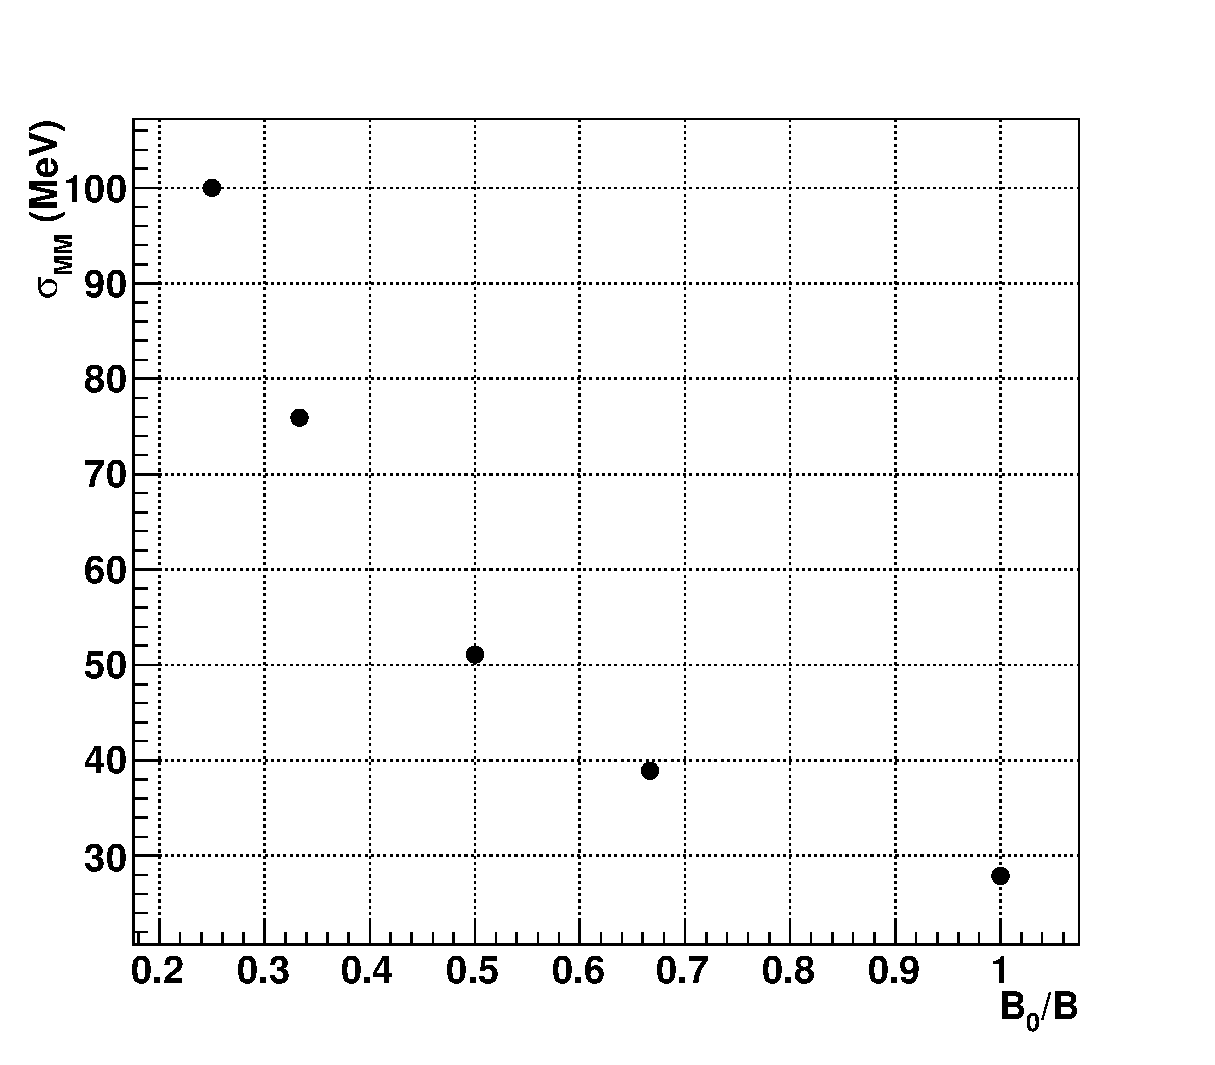
\includegraphics[width=0.45\textwidth]{resPfield.eps}}
\caption{\footnotesize \label{fig:4} Left: reconstructed $J/\psi$ mass resolution as a function of the CLAS12 toroidal field intensity (normalized to the maximum possible value). Right: resolution on the missing mass on the $e^+\,e^-$ pair as a function of the CLAS12 toroidal field intensity.}
\end{figure}

The CLAS12 acceptance, as a function of the $J/\psi\, p$ invariant mass $W$, is reported in Fig.~\ref{fig:5}, for both measurement strategies outlined below. For both cases, the acceptance shows a smooth increase with $W$, with an average value of $\simeq 13\%$ for the detection of all final state particles ($\simeq 16\%$ for the detection of the $e^{+} e^{-}$ pair only). We observe that the ``deep'' at $W=4.4$ GeV, at the resonance mass, is due to the fact that resonance production mechanism is characterized by a very different kinematics than the background, in particular for the $t$ dependence, and, therefore, the corresponding CLAS12 response is different. 

We also investigated the effect of a change in the CLAS12 toroidal field, finding a very modest dependence on in. 
The larger effect comes from inverting the polarity of the field, i.e. having the proton being inbended by the field. In this case, the acceptance for the measure of all the final state particles drops to $\simeq 9\%$, while there is no effect to the acceptance for the measure of the $e^+ e^-$ pair only.

\begin{figure}[tpb]
\center
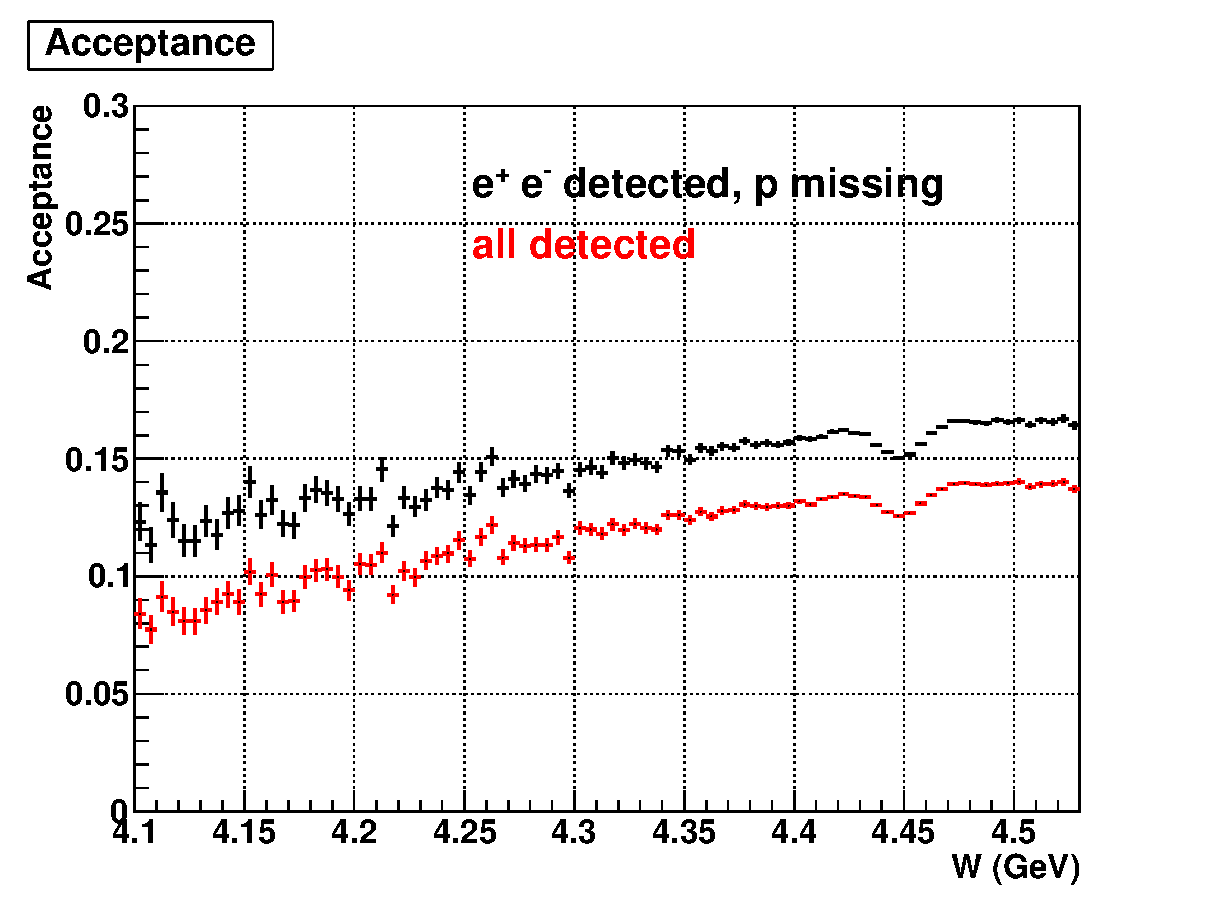
\includegraphics[width=0.7\textwidth]{acceptanceNominal.eps}
\caption{\footnotesize \label{fig:5} Detector acceptance as a function of the  $J/\psi\, p$ invariant mass, for both measurement strategies outlined before. Both plots refer to the maximum value of the CLAS12 toroidal field, configured to have positive particles outbending. }
\end{figure}

Finally, the resolution on the $J/\psi\, p$ invariant mass $W$, \textit{measured as the missing mass on the low-angle scattered electron}, is shown in Fig.~\ref{fig:6}. As pointed before, this quantity depends only on the measurement of the final state electron with the Forward Tagger calorimeter, and it is almost insensitive to the CLAS12 configuration. For $W=4.4$ GeV, $\sigma_W=5.5$ MeV, in agreement with the previous estimate.

\begin{figure}[tpb]
\center
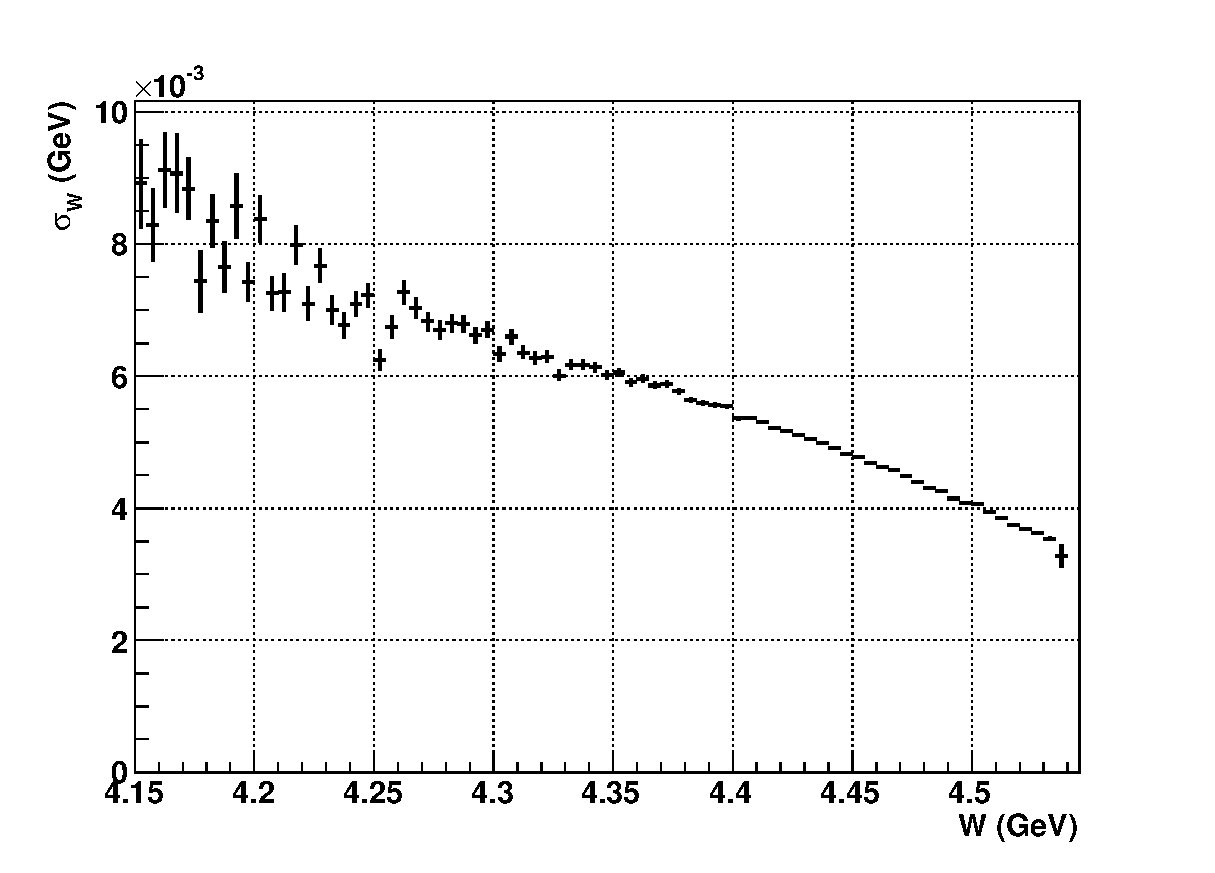
\includegraphics[width=0.7\textwidth]{resolutionW.eps}
\caption{\footnotesize \label{fig:6} Resolution on the  $J/\psi\, p$ invariant mass.}
\end{figure}


\section{Conclusions and outlook}

In this note, we briefly discussed the feasibility of the measurement of the $\gamma^* p \rightarrow J/\psi \, p$ reaction in the MesonEx experiment at Jefferson Laboratory, searching for resonances in the $J/\psi\,p$ system. 

In particular, we showed that, with the CLAS12 + Forward Tagger system, it is possible to reach a resolution on the $J/\psi \, p$ system $W$ of 5.5 MeV for $W=4.4$ GeV, with an acceptance of $\simeq 13\%$, if all the final state particles (proton and $e^+ e^-$ pair) are measured in coincidence with the low-angle scattered electron. 
 
These results encourage a further study of this reaction within the experiment. In the following, we just mention further points that should be addressed.
\begin{itemize}
\item{In this note, we just focused on the $P_c(4440)$ state reported by LHCB, considering the $J^P$ assignment $(3/2)^-$. However, the sensitivity of the experiment to a resonance signal should be studied as a function of the mass and width. Furthermore, the possibility of uniquely determining the resonance quantum numbers trough a Partial Wave Analysis should be investigated, in particular taking into account the polarization of the virtual photon beam.}
\item{A study of the possible backgrounds associated with this reaction should be performed, in order to determine the sensitivity of the experiment to the resonance production cross-section. This would also permit to identify the best measurement strategy between the two cases discussed in this note.}
\end{itemize}  

\appendix
\section{Model for the reaction $\gamma p \rightarrow J/\psi \, p \rightarrow e^+ e^- p$ }\label{app:model}

In this appendix, we describe the analytical model developed for amplitude of the reaction $\gamma p \rightarrow J/\psi \, p \rightarrow e^+ e^-  p$. Two separate contribution were considered: the production of an $s-$channel resonance $X$ (signal), and a non-resonant production mechanism, parametrized via the $t-$channel exchange of a Pomeron trajectory (background). These two contributions were added incoherently in the total cross-section.

It is worth to underline that here we only discuss the amplitude for the real photo-production process $\gamma p \rightarrow J/\psi$. The connection to the quasi-real photoproduction reaction (low $Q^2$ electron-scattering) that is actually measured in MesonEx is reported, for example, in \cite{mythesis}.

\subsection{Signal}

The Lorentz-invariant amplitude for the reaction  $\gamma p \rightarrow J/\psi \, p$ depends on both $s$, the total energy squared in the center of mass frame, and $t$, the total momentum transferred squared. It can be expanded in terms of partial waves as (\cite{Agashe:2014kda}, eq. 46.6):

\begin{equation}
M_{\lambda_\gamma,\lambda_p}^{\lambda_\psi,\lambda_{p^{\prime}}} (s,t) = \sum_J (2J+1)_JM_{\lambda_\gamma,\lambda_p}^{\lambda_\psi,\lambda_{p^{\prime}}} (s) {D^{J*}_{\lambda_\gamma - \lambda_p, \lambda_\psi-\lambda_{p^\prime}}}(\phi,\theta,-\phi) \; \; \; ,
\end{equation}
where $\lambda_\gamma$, $\lambda_p$, $\lambda_\psi$, $\lambda_p^{\prime}$ are, respectively, the helicities of the incoming photon, target proton, final state $J/\psi$ and final state proton. $D^J_{\lambda_\gamma - \lambda_p, \lambda_\psi-\lambda_{p^\prime}}(\phi,\theta,-\phi)$ is a Wigner $D-$function, with $\theta$ and $\phi$ the $J/\psi$ scattering angles measured in the CM frame, and the initial state photon momentum aligned along the $+z$ axis.
$_JM_{\lambda_\gamma,\lambda_p}^{\lambda_\psi,\lambda_{p^{\prime}}} (s)$ is a reduced amplitude for the $J-$th partial wave, that depends only on $s$.

For the case of the production of a single $s-$channel resonances, with defined spin $J$, the above sum simplifies to:
\begin{equation}
M_{\lambda_\gamma,\lambda_p}^{\lambda_\psi,\lambda_{p^{\prime}}} (s,t) = (2J+1)_JM_{\lambda_\gamma,\lambda_p}^{\lambda_\psi,\lambda_{p^{\prime}}} (s) {D^{J*}_{\lambda_\gamma - \lambda_p, \lambda_\psi-\lambda_{p^\prime}}}(\phi,\theta,-\phi) \; \; \; ,
\end{equation}

If there is only a single resonance present and all relevant thresholds are far away, a Breit-Wigner approximation can be used for $_JM$ (\cite{Agashe:2014kda}, eq. 46.22):

\begin{equation}
_JM_{\lambda_\gamma,\lambda_p}^{\lambda_\psi,\lambda_{p^{\prime}}} (s) = - \frac{g^{\lambda_\gamma,\lambda_p}_{I} g^{\lambda_\psi,\lambda_{p^\prime}}_{F}}{s-M^2+i\sqrt{s}\Gamma} \; \; \; ,
\end{equation}
where $M$, $\Gamma$ are the resonance mass and total width, and $g^{\lambda_\gamma,\lambda_p}_{I}$ and $g^{\lambda_\psi,\lambda_{p^{\prime}}}_{F}$ are, respectively, the resonance coupling to the initial $\gamma p$ state and to the final $J/\psi p^{\prime}$ state, that explicitly depend on the helicity states of the external particles.

In general, for the reaction  $\gamma p \rightarrow X \rightarrow J/\psi \, p$, there are 4 unknown  helicity couplings $g_I$ and 6 unknown  helicity couplings $g_F$, given the different helicity configurations that are possible for the initial and final state. However, both the processes $X \rightarrow \gamma p$ (EM interaction) and $X \rightarrow J/\psi \, p$ (strong interaction) conserve parity. Therefore, assuming $J^P=(3/2)^-$ quantum numbers for the $X$ state, the following constraints apply (see, for example, \cite{Richman:1984gh}) :
\begin{eqnarray}
g^{\lambda_\gamma,\lambda_p}_{I} &=& g^{-\lambda_\gamma,-\lambda_p}_{I} \\
g^{\lambda_\psi,\lambda_p^\prime}_{F} &=& g^{-\lambda_\psi,-\lambda_{p^\prime}}_{F}
\end{eqnarray}
This reduces the total number of unknown helicity couplings from 10 to 5 (2 for the initial state, 3 for the final state).

To further reduce the number of unknown helicity couplings, we made the following two assumptions:

\begin{itemize}
\item{We make use of ``vector meson dominance'' \cite{Bauer:1977iq} to relate each initial-state coupling  $g^{\lambda_\gamma,\lambda_p}_{I}$ to the corresponding final-state one $g^{\lambda_\psi,\lambda_{p^{\prime}}}_{F}$. We assume that, since the $X$ state couples to the $J/\psi p$ state, the EM interaction with the $\gamma p$ state proceeds trough the $J/\psi$ pole. We write the coupling between the photon and vector mesons as:
\begin{equation}
\mathcal{L}=\sum_V \frac{e M^2_V}{f_v} V_\mu A^{\mu} \; \; \; ,
\end{equation} 
where the effective coupling constant $e / f_v$ can be related to the partial width $\Gamma^V_{ee}$ of the EM decay process $V\rightarrow e^+ e^-$:
\begin{equation}
\frac{e}{f_V}=\left(\frac{3\Gamma^V_{ee}}{\alpha M}\right)^{1/2}
\end{equation}
}
For the $J/\psi$ meson, $\Gamma^V_{ee} = 5.55$ keV, therefore $e/f = 2.714\cdot 10^{-2}$.

With this assumption, we write:
\begin{equation}
g^{\lambda_a,\lambda_b}_{I}=(e/f) g^{\lambda_a,\lambda_b}_{F} \; \; \; ,
\end{equation}
were we explicitly reported the helicities of the particles to underline that this relation holds separately for each configuration. With this assumption, the 2 initial-state couplings not fixed by parity conservation are fixed by the corresponding final-state ones, leaving only these as free parameters.

\item{A further reduction of the helicity couplings $g^{\lambda_\psi,\lambda_{p^{\prime}}}_{F}$ can be achieved by relating them to the ``spherical-base'' couplings $B_{LS}$, and then restricting the possible values of the orbital angular momentum $L$ for the decay $X\rightarrow J/\psi p$. 
The relation between the two basis, expressed via Clebsh-Gordan coefficients reads:
\begin{equation}
g^{\lambda_\psi,\lambda_{p^{\prime}}}_{F} =\sum_{L,S} B^{J}_{L,S} \sqrt\frac{2L+1}{2J+1} (1 \, \lambda_\psi ; 1/2 \,  \lambda_{p^\prime} | S \lambda_\psi - \lambda_{p^{\prime}}) (L  \,0 ; S  \, \lambda_\psi - \lambda_{p^{\prime}} | J \lambda_\psi - \lambda_{p^{\prime}})
\end{equation}


For this process, the total spin $S$ of the daughers can be either 1/2 or 3/2 and, correspondingly, the orbital angular momentum $L$ can be 1 or 2 (for the $S=1/2$ case) or 0 $\ldots$ 3 for the $S=3/2$ case.
We make the assumption that, due to the reduced phase-space available to the decay process, angular barrier effects reduce the possible values of $L$ only to the lowest possible value $L=0$, and, correspondingly, $S=3/2$.

The relation between the helicity coupling $g^{\lambda_\psi,\lambda_{p^{\prime}}}_{F}$ and the corresponding ``spherical-base'' coupling, therefore, reduces to:
\begin{equation}
g^{\lambda_\psi,\lambda_{p^{\prime}}}_{F} =\frac{1}{2} B_{0,3/2} (1 \, \lambda_\psi ; 1/2 \,  \lambda_{p^\prime} | 3/2 \lambda_\psi - \lambda_{p^{\prime}})
\end{equation}
}
This gives:
\begin{eqnarray}
g^{1,+}_{F}=g^{-1,-}_F&=&\frac{1}{2}B_{0,3/2}\frac{1}{\sqrt{3}}\\
g^{1,-}_{F}=g^{-1,+}_F&=&\frac{1}{2}B_{0,3/2} = \sqrt{3}g^{1,+}\\
g^{0,+}_F=g^{0,-}_F&=&\frac{1}{2}B_{0,3/2}\sqrt{\frac{2}{3}}=\sqrt{2}g^{1,+}
\end{eqnarray}
\end{itemize}

In conclusion, \textbf{all} the unknown helicity couplings $g_i$, $g_f$ are related, by the above equations, to the single unknown $g^{1,+}_{F}$ that, in turns, fix the total cross-section intensity.
 
This is given by (assuming no polarization for the initial state particles):
\begin{equation}
d\sigma = \frac{1}{4} \sum_{\lambda} \frac{d\Omega}{(8\pi)^2}\frac{1}{s}\frac{p_f(s)}{p_i(s)} 16 |M^\lambda(s)D^{3/2*}_{\lambda}(\phi,\theta,-\phi)|^2  \; \; \; ,
\end{equation}
where we used the compact notation $\lambda={\lambda_\gamma,\lambda_p,\lambda_\psi,\lambda_{p^\prime}}$ to indicate the sum over the polarizations. $p_f(s)$ and $p_i(s)$ are, respectively, the magnitude of the 3-momentum of the final and initial state particles in the CM frame.

Integrating over $\Omega$, this gives:
\begin{equation}
\sigma = \frac{1}{16\pi s}\frac{p_f(s)}{p_i(s)}\frac{1}{(s-M^2)^2+s\Gamma^2}\sum_{\lambda_I,\lambda_F}(g_I^{\lambda_i}g_F^{\lambda_F})^2 = 
\frac{96}{16\pi s}\frac{p_f(s)}{p_i(s)}\frac{1}{(s-M^2)^2+s\Gamma^2} (e/f)^2 (g_F^{1,+})^4
\end{equation}
The coupling $g_F^{1,+}$ can be related to the partial width $\Gamma_F$ for the decay process $X \rightarrow J/\psi p$ by using the relation (\cite{Agashe:2014kda}, eq. 46.16 and eq. 46.21):
\begin{equation}
\Gamma_F(s)=\frac{p_f}{8 \pi s}g^2_F \; \; , \; \; g^2_F \equiv \sum_{\lambda_F}(g^{\lambda_F})^2 = 12 (g^{1,+}_F)^2
\end{equation}
Therefore:
\begin{equation}
\sigma = \frac{8\pi}{3} \frac{s}{p_i p_f}(e/f)^2\frac{\Gamma^2_F}{(s-M^2)^2+\Gamma^2 s} 
\end{equation}
At there resonance peak, $s=M^2$, this gives:
\begin{equation}
\sigma(M) = \frac{8\pi}{3}(e/f)^2\frac{1}{p_ip_f} B^2_F \; \; \; ,
\end{equation}
where the branching franction $BR=\Gamma_F / \Gamma$ has been introduced. Specifically, for the $X(4449.8)$ state, this gives $\sigma(M)\simeq 1.3 \cdot BR^2 \, \mu$barn

\subsection{Background}

We parametrized the non-resonant $J/\psi$ production mechanism using Regge theory, namely via the $t-$channel exchange of a Pomeron trajectory. The free parameters (trajectory parameters and vertex functions) were tuned to reproduce the experimental data measured at higher energy ($E_\gamma > $  13 GeV, \cite{Camerini:1975cy}).
Specifically, the simplified amplitude we used reads:
\begin{equation}
M_{\lambda_\gamma,\lambda_p}^{\lambda_\psi,\lambda_{p^{\prime}}} = \left(\frac{s}{s_0}\right)^{\alpha_P(t)} \beta_{\lambda_\gamma,\lambda_\psi}\beta_{\lambda_p,\lambda_{p^\prime}} e^{-b|t|} \; \; \; ,
\end{equation}
where $\alpha_P(t)$ is the Pomeron trajectory, parametrized as $\alpha_P(t)=\alpha_0+\alpha^{\prime}(t)$. $\beta_{\lambda_\gamma,\lambda_{psi}}$, $\beta_{\lambda_p,\lambda_{p^{\prime}}}$ are, respectively, the Pomeron-photon-$J/\psi$ coupling and the Pomeron-proton-proton coupling. The term $e^{-b|t|}$ is an ``effective'' form factor, that accounts for both vertexes.

By parity conservation, considering the $0^{++}$ quantum numbers associated with the Pomeron trajectory, the following relations hold:
\begin{eqnarray}
\beta_{\lambda_\gamma,\lambda_{\psi}}&=&\beta_{-\lambda_\gamma,-\lambda_{\psi}}\\
\beta_{\lambda_p,\lambda_{p^{\prime}}}&=&\beta_{-\lambda_p,-\lambda_{p^{\prime}}}
\end{eqnarray}
To further reduce the number of independent couplings to a single term $\beta_0$, we made the following assumptions:
\begin{itemize}
\item{The polarization of the incoming photon is entirely transferred to the final state $J/\psi$. The only non-zero couplings, therefore, are those with $\lambda_\gamma=\lambda_{\psi}$, i.e. $\beta_{1,1}=\beta_{-1,-1}$. As a consequence, no linearly polarized $J/\psi$ are produced in the process.}
\item{No spin-flip mechanism is allowed at the proton vertex, given the zero-spin nature of the Pomeron trajectory.}
\end{itemize}

The corresponding differential cross-section, already averaged over the initial state helicities and summed over the final state ones, is:
\begin{equation}\label{eq:dsigma}
\frac{d\sigma}{dt}=\frac{1}{64\pi s}\frac{1}{p_i^2} \beta_0^2  \left(\frac{s}{s_0}\right)^{2\alpha_P(t)} e^{-2b|t|} \; \; \; ,
\end{equation}
so that, at fixed $s$, the $t-$dependence reads:
\begin{equation}
\frac{d\sigma}{dt} \propto e^{-2|t|(b+\alpha^\prime\cdot\ln(s/s0))}
\end{equation}

To fix the free parameters ($s_0$, $\beta$, $b$, $\alpha_0$ and $\alpha^{\prime}$) we proceeded as follows. We started by fixing $s_0$ and $\alpha_{\prime}$ to their ``nominal'' value (1 GeV$^2$ and 0.25). The latter value to a ``soft Pomeron'', that is expected to give the largest contribution to the cross-section at low $s$ values \cite{Adloff:2000vm}. Then, we tuned the value of $\beta$ to reproduce the $t-$dependence reported by Camerini et al. \cite{Camerini:1975cy}, in a slightly higher $s$ range. We used $\beta=0.7$, corresponding to a $t-$slope of $\simeq$2.8 at $s\simeq$16 GeV$^2$. 
Finally, we performed a best fit to the available $\sigma(s)$ data to fix $\alpha_0$ and $\beta$ (see Fig.~\ref{fig:bck}). We got $\alpha_0=2.2$ and $\beta=4.36\cdot10^{-4}$.
\begin{figure}
\centering
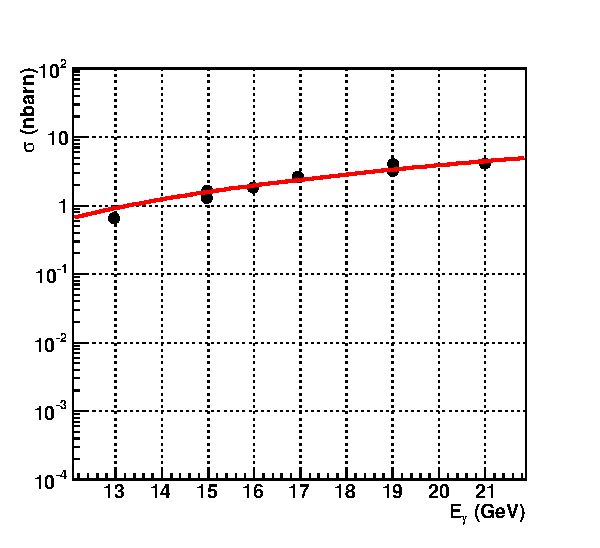
\includegraphics[width=.6\textwidth]{bck.eps}
\caption{\small\label{fig:bck} Total cross-section as a function of the incoming photon energy for the non-resonant process  $\gamma p \rightarrow J/\psi \, p$. The black points are experimental data from \cite{Camerini:1975cy}, while the red curve is the best with performed with eq.~\ref{eq:dsigma}.}

\end{figure}








\subsection{$J/\psi \rightarrow e^+ e^-$ decay}

So far, both for the signal and for the background terms, we considered the reaction  $\gamma p \rightarrow J/\psi \, p$, i.e. we threated the $J/\psi$ meson as a final state particle, measured with the detector. However, the reaction that is \textit{actually} measured includes the decay process $J/\psi \rightarrow e^+ e^-$. Therefore, both amplitudes introduced before need to be modified to include this, as follows. The $J/\psi$ helicity $\lambda_\psi$ is no longer an \textit{external} index, summed incoherently at the cross-section level, but becomes an \textit{internal} index, summed coherently at the amplitude level. Contemporary, the two helicities $\lambda_+$ and $\lambda_-$ for the positron and the electron are introduced.

The full amplitude reads:
\begin{equation}
M_{\lambda_\gamma,\lambda_p}^{\lambda_+,\lambda_-,\lambda_{p^{\prime}}} = \sum_{\lambda_\psi} M_{\lambda_\gamma,\lambda_p}^{\lambda_\psi,\lambda_{p^{\prime}}}(\gamma p \rightarrow J/\psi p) \cdot M_{\lambda_\psi}^{\lambda_+,\lambda_-}(J/\psi \rightarrow e^+ e^-)
\end{equation}
The amplitude for the process $J/\psi \rightarrow e^+ e^-$ reads:
\begin{equation}
M_{\lambda_\psi}^{\lambda_+,\lambda_-} = g^{1}_{\lambda_-,\lambda_+}D^{1*}_{\lambda_\psi,\lambda_--\lambda_+}(\phi_2,\theta_2,-\phi_2) \; \; \; ,
\end{equation}
where the $\theta_2$, $\phi_2$ angles define the orientation of the $e^-$ 3-momentum in the $J/\psi$ rest frame, with the $z$ axis aligned along the $J/\psi$ momentum in the CM frame.
Again, applying parity conservation to the decay, one gets $g_{\lambda_a,\lambda_b}=g_{-\lambda_,-\lambda_b}$, reducing to 2 the number of independent decay couplings. Furthermore, since the $e^+$ and the $e^-$ in the decay are ultra-relativistic, the combination $\Delta_\lambda \equiv \lambda_--\lambda_+$ can only be $+1$ or $-1$, but not 0 (i.e. $g^1_{\lambda_-=\lambda_+}=0$). Therefore, there is only one free coupling for the decay process, $g^1_{\delta_\lambda=1} = g^1_{\delta_\lambda=-1} \equiv g^1$. 
This can be re-absorbed in the production amplitude, giving: 
\begin{equation}
M_{\lambda_\psi}^{\lambda_+,\lambda_-} = D^{1*}_{\lambda_\psi,\lambda_--\lambda_+}(\phi_2,\theta_2,-\phi_2) 
\end{equation}
\begin{thebibliography}{9}
\bibitem{Aaij:2015tga} 
  R.~Aaij {\it et al.} [LHCb Collaboration],
  %``Observation of $J/\psi p$ resonances consistent with pentaquark states in ${\Lambda_b^0\to J/\psi K^-p}$ decays,''
  Phys.\ Rev.\ Lett.\  {\bf 115}, 072001 (2015)
  [arXiv:1507.03414 [hep-ex]].
  %%CITATION = ARXIV:1507.03414;%%
  %24 citations counted in INSPIRE as of 14 Aug 2015

\bibitem{Chen:2015loa} 
  R.~Chen, X.~Liu, X.~Q.~Li and S.~L.~Zhu,
  %``A new page for hadron physics: Identifying exotic hidden-charm pentaquarks,''
  arXiv:1507.03704 [hep-ph].
  %%CITATION = ARXIV:1507.03704;%%
  %13 citations counted in INSPIRE as of 14 Aug 2015

\bibitem{Chen:2015moa} 
  H.~X.~Chen, W.~Chen, X.~Liu, T.~G.~Steele and S.~L.~Zhu,
  %``Towards exotic hidden-charm pentaquarks in QCD,''
  arXiv:1507.03717 [hep-ph].
  %%CITATION = ARXIV:1507.03717;%%
  %10 citations counted in INSPIRE as of 14 Aug 2015

\bibitem{Roca:2015dva} 
  L.~Roca, J.~Nieves and E.~Oset,
  %``The LHCb pentaquark as a $\bar{D}^*\Sigma_c-\bar{D}^*\Sigma_c^*$ molecular state,''
  arXiv:1507.04249 [hep-ph].
  %%CITATION = ARXIV:1507.04249;%%
  %13 citations counted in INSPIRE as of 14 Aug 2015


\bibitem{He:2015cea} 
  J.~He,
  %``The $\bar{D}\Sigma^*_c$ and $\bar{D}^*\Sigma_c$ interactions and the LHCb hidden-charmed pentaquarks,''
  arXiv:1507.05200 [hep-ph].
  %%CITATION = ARXIV:1507.05200;%%
  %7 citations counted in INSPIRE as of 14 Aug 2015


\bibitem{Maiani:2015vwa} 
  L.~Maiani, A.~D.~Polosa and V.~Riquer,
  %``The New Pentaquarks in the Diquark Model,''
  arXiv:1507.04980 [hep-ph].
  %%CITATION = ARXIV:1507.04980;%%
  %9 citations counted in INSPIRE as of 14 Aug 2015


\bibitem{Anisovich:2015cia} 
  V.~V.~Anisovich, M.~A.~Matveev, J.~Nyiri, A.~V.~Sarantsev and A.~N.~Semenova,
  %``Pentaquarks and resonances in the $pJ/\psi$ spectrum,''
  arXiv:1507.07652 [hep-ph].
  %%CITATION = ARXIV:1507.07652;%%
  %6 citations counted in INSPIRE as of 14 Aug 2015




\bibitem{Lebed:2015tna} 
  R.~F.~Lebed,
  %``The Pentaquark Candidates in the Dynamical Diquark Picture,''
  arXiv:1507.05867 [hep-ph].
  %%CITATION = ARXIV:1507.05867;%%
  %7 citations counted in INSPIRE as of 14 Aug 2015

\bibitem{Meissner:2015mza} 
  U.~G.~Meißner and J.~A.~Oller,
  %``Testing the $\chi_{c1}\, p$ composite nature of the $P_c(4450)$,''
  arXiv:1507.07478 [hep-ph].
  %%CITATION = ARXIV:1507.07478;%%
  %5 citations counted in INSPIRE as of 14 Aug 2015

\bibitem{Guo:2015umn} 
  F.~K.~Guo, U.~G.~Meißner, W.~Wang and Z.~Yang,
  %``How to reveal the exotic nature of the P_c(4450),''
  arXiv:1507.04950 [hep-ph].
  %%CITATION = ARXIV:1507.04950;%%
  %9 citations counted in INSPIRE as of 14 Aug 2015

\bibitem{Liu:2015fea} 
  X.~H.~Liu, Q.~Wang and Q.~Zhao,
  %``Understanding the newly observed heavy pentaquark candidates,''
  arXiv:1507.05359 [hep-ph].
  %%CITATION = ARXIV:1507.05359;%%
  %9 citations counted in INSPIRE as of 14 Aug 2015

\bibitem{Mikhasenko:2015vca} 
  M.~Mikhasenko,
  %``A triangle singularity and the LHCb pentaquarks,''
  arXiv:1507.06552 [hep-ph].
  %%CITATION = ARXIV:1507.06552;%%
  %6 citations counted in INSPIRE as of 14 Aug 2015


\bibitem{Karliner:2015voa} 
  M.~Karliner and J.~L.~Rosner,
  %``Photoproduction of Exotic Baryon Resonances,''
  arXiv:1508.01496 [hep-ph].
  %%CITATION = ARXIV:1508.01496;%%
  %1 citations counted in INSPIRE as of 14 Aug 2015

\bibitem{Wang:2015jsa} 
  Q.~Wang, X.~H.~Liu and Q.~Zhao,
  %``Photoproduction of hidden charm pentaquark states $P_c^+(4380)$ and $P_c^+(4450)$,''
  arXiv:1508.00339 [hep-ph].
  %%CITATION = ARXIV:1508.00339;%%
  %3 citations counted in INSPIRE as of 14 Aug 2015
\bibitem{Kubarovsky:2015aaa} 
  V.~Kubarovsky and M.~B.~Voloshin,
  %``Formation of hidden-charm pentaquarks in photon-nucleon collisions,''
  arXiv:1508.00888 [hep-ph].
  %%CITATION = ARXIV:1508.00888;%%
  %2 citations counted in INSPIRE as of 14 Aug 2015
\bibitem{MesonEx}
M.~Battaglieri\textit{ et al.} (CLAS collaboration),
``Meson Spectrsocopy with low $Q^2$ electron scattering in CLAS12'',
Proposal to Jefferson Laboratory PAC37 (2011).


\bibitem{Celentano:2014boa} 
  A.~Celentano [CLAS Collaboration],
  %``The Forward Tagger facility for low $Q^2$ experiments at Jefferson Laboratory,''
  EPJ Web Conf.\  {\bf 73}, 08004 (2014).
  %%CITATION = 00776,73,08004;%%
  %1 citations counted in INSPIRE as of 14 Aug 2015

\bibitem{Budnev:1974de} 
  V.~M.~Budnev, I.~F.~Ginzburg, G.~V.~Meledin and V.~G.~Serbo,
  %``The Two photon particle production mechanism. Physical problems. Applications. Equivalent photon approximation,''
  Phys.\ Rept.\  {\bf 15}, 181 (1975).
  %%CITATION = PRPLC,15,181;%%
  %958 citations counted in INSPIRE as of 14 Aug 2015
\bibitem{Camerini:1975cy} 
  U.~Camerini {\it et al.},
  %``Photoproduction of the psi Particles,''
  Phys.\ Rev.\ Lett.\  {\bf 35}, 483 (1975).
  %%CITATION = PRLTA,35,483;%%
  %174 citations counted in INSPIRE as of 17 Aug 2015

\bibitem{Brodsky:2000zc} 
  S.~J.~Brodsky, E.~Chudakov, P.~Hoyer and J.~M.~Laget,
  %``Photoproduction of charm near threshold,''
  Phys.\ Lett.\ B {\bf 498}, 23 (2001)
  [hep-ph/0010343].
  %%CITATION = HEP-PH/0010343;%%
  %34 citations counted in INSPIRE as of 17 Aug 2015

\bibitem{mythesis}
  A.~Celentano, ``The Forward Tagger detector for CLAS12 at Jefferson Laboratory and the MesonEx experiment'', PhD thesis.


\bibitem{Agashe:2014kda} 
  K.~A.~Olive {\it et al.} [Particle Data Group Collaboration],
  %``Review of Particle Physics,''
  Chin.\ Phys.\ C {\bf 38}, 090001 (2014).
  %%CITATION = CHPHD,C38,090001;%%
  %1713 citations counted in INSPIRE as of 24 août 2015
\bibitem{Richman:1984gh} 
  J.~D.~Richman,
  %``An Experimenter's Guide to the Helicity Formalism,''
  CALT-68-1148.
  %%CITATION = CALT-68-1148;%%
  %38 citations counted in INSPIRE as of 24 août 2015
\bibitem{Bauer:1977iq} 
  T.~H.~Bauer, R.~D.~Spital, D.~R.~Yennie and F.~M.~Pipkin,
  %``The Hadronic Properties of the Photon in High-Energy Interactions,''
  Rev.\ Mod.\ Phys.\  {\bf 50}, 261 (1978)
  [Rev.\ Mod.\ Phys.\  {\bf 51}, 407 (1979)].
  %%CITATION = RMPHA,50,261;%%
  %802 citations counted in INSPIRE as of 24 août 2015
\bibitem{Adloff:2000vm} 
  C.~Adloff {\it et al.} [H1 Collaboration],
  %``Elastic photoproduction of J / psi and Upsilon mesons at HERA,''
  Phys.\ Lett.\ B {\bf 483}, 23 (2000)
  [hep-ex/0003020].
  %%CITATION = HEP-EX/0003020;%%
  %191 citations counted in INSPIRE as of 24 août 2015

\end{thebibliography}
\end{document}

